\documentclass[11pt]{article}

\usepackage[margin=1.1in]{geometry}
\usepackage{amsmath,amssymb,amsthm}
\usepackage{graphicx}
\usepackage{booktabs}
\usepackage{microtype}
\usepackage[round]{natbib}
\usepackage{xcolor}
\usepackage[colorlinks=true,linkcolor=blue!50!black,citecolor=blue!50!black,urlcolor=blue!50!black]{hyperref}

\graphicspath{{figures/}}
% generated by ceiling.py -- do not edit
\newcommand{\chTotalB}{6.2}
\newcommand{\chZips}{2{,}232}
\newcommand{\chReps}{72}
\newcommand{\chRealReps}{71}
\newcommand{\chComponents}{4}
\newcommand{\chTargetB}{1}
\newcommand{\chKAtTarget}{6}
\newcommand{\chKPlusOne}{7}
\newcommand{\chSizeAtKPlusOne}{886}
\newcommand{\chBinaries}{13{,}392}
\newcommand{\chRepRatio}{12}
\newcommand{\chEvenLabel}{even-ish}
\newcommand{\chEvenSplit}{2 / 2.2 / 1.1 / 0.9}
\newcommand{\chEvenkSix}{19.4}
\newcommand{\chEvenkSixAlloc}{2/2/1/1}
\newcommand{\chEvenkSixMin}{0.90}
\newcommand{\chEvenkSixMax}{1.10}
\newcommand{\chEvenkSeven}{41.4}
\newcommand{\chEvenkSevenAlloc}{2/3/1/1}
\newcommand{\chEvenkSevenMin}{0.73}
\newcommand{\chEvenkSevenMax}{1.10}
\newcommand{\chEvenkEight}{55.9}
\newcommand{\chEvenkEightAlloc}{3/3/1/1}
\newcommand{\chEvenkEightMin}{0.67}
\newcommand{\chEvenkEightMax}{1.10}
\newcommand{\chEvenBestK}{6}
\newcommand{\chEvenBestSpread}{19.4}
\newcommand{\chEastLabel}{east-heavy}
\newcommand{\chEastSplit}{1.6 / 3 / 0.9 / 0.7}
\newcommand{\chEastkSix}{87.1}
\newcommand{\chEastkSixAlloc}{1/3/1/1}
\newcommand{\chEastkSixMin}{0.70}
\newcommand{\chEastkSixMax}{1.60}
\newcommand{\chEastkSeven}{33.9}
\newcommand{\chEastkSevenAlloc}{2/3/1/1}
\newcommand{\chEastkSevenMin}{0.70}
\newcommand{\chEastkSevenMax}{1.00}
\newcommand{\chEastkEight}{25.8}
\newcommand{\chEastkEightAlloc}{2/4/1/1}
\newcommand{\chEastkEightMin}{0.70}
\newcommand{\chEastkEightMax}{0.90}
\newcommand{\chEastBestK}{8}
\newcommand{\chEastBestSpread}{25.8}
\newcommand{\chCoastLabel}{coast-heavy}
\newcommand{\chCoastSplit}{2.6 / 2.6 / 0.6 / 0.4}
\newcommand{\chCoastkSix}{87.1}
\newcommand{\chCoastkSixAlloc}{2/2/1/1}
\newcommand{\chCoastkSixMin}{0.40}
\newcommand{\chCoastkSixMax}{1.30}
\newcommand{\chCoastkSeven}{101.6}
\newcommand{\chCoastkSevenAlloc}{3/2/1/1}
\newcommand{\chCoastkSevenMin}{0.40}
\newcommand{\chCoastkSevenMax}{1.30}
\newcommand{\chCoastkEight}{60.2}
\newcommand{\chCoastkEightAlloc}{3/3/1/1}
\newcommand{\chCoastkEightMin}{0.40}
\newcommand{\chCoastkEightMax}{0.87}
\newcommand{\chCoastBestK}{8}
\newcommand{\chCoastBestSpread}{60.2}
\newcommand{\chEastkSixMinSpread}{77.4}
\newcommand{\chEastkSixMinAlloc}{2/2/1/1}
\newcommand{\chCone}{0.70}
\newcommand{\chCtwo}{0.28}
\newcommand{\chCgap}{0.42}
\newcommand{\chSat}{5}
\newcommand{\chUown}{0.335}
\newcommand{\chUother}{0.314}
\newcommand{\chOppShare}{89.6}
\newcommand{\chPremShare}{6.3}
\newcommand{\chUswing}{6.7}
\newcommand{\chMatchUtilDiag}{101}
\newcommand{\chMatchUtilAnti}{100}
\newcommand{\chMatchNashDiag}{4.605}
\newcommand{\chMatchNashAnti}{6.802}


\newtheorem{prop}{Proposition}
\newtheorem{cor}[prop]{Corollary}
\newtheorem{obs}{Observation}
\theoremstyle{definition}
\newtheorem{example}{Example}
\newtheorem{remark}{Remark}

\newcommand{\Sfree}{S_{\mathrm{free}}}
\newcommand{\cfree}{c_{\mathrm{free}}}
\newcommand{\owner}{\operatorname{own}}

\title{Balanced districting for a national sales channel:\\
the model, the two-stage scheme, and the balance ceiling}
\author{Territory-division project\thanks{A self-contained companion to
\texttt{nash\_territory\_division.tex} and to
\texttt{research/contiguity/math\_note/math\_note.tex}, which treats the two-player
merger problem this note re-scopes. The source of record is
\texttt{research/contiguity/NWAY.md}; the implementations are
\texttt{td/model.py} and \texttt{td/channel.py}, with
\texttt{battery/code/tests/test\_nway.py} and \texttt{test\_channel.py} asserting the
identities proved below. Every number in Section~\ref{sec:ceiling} and in the
saturation arithmetic of Section~\ref{sec:decomp} is computed by \texttt{ceiling.py}
and injected as a macro, never transcribed.}}
\date{2026-08-31}

\begin{document}
\maketitle

\begin{abstract}
\noindent
The territory problem has been re-scoped. Instead of dividing a contested region between
two legacy representatives of merging firms, the business is standing up a
\emph{new} ``national'' channel --- the two largest product manufacturers carved out of
the financial-institutions and wirehouse channels --- and wants it cut into territories
of roughly equal market opportunity. This note develops the mathematics of that problem.
We generalise the utility model to $n$ representatives per postal code and show it
reduces identically to the two-player model at $n=2$; we prove the model is invariant
under a global rescaling of the dollar fields, which licenses exporting a descaled
instance from the confidential machine; we prove the central structural fact, that
\emph{maximum Nash welfare on a common measure is exactly equal-size districting}, so the
${\sim}\$\chTargetB$B target is an emergent property rather than a constraint; we
decompose total welfare into a partition-invariant part and an incumbency premium, and
size the two on real saturation; and we prove that a \emph{disconnected} footprint --- the
channel covers the two coasts, Texas and Florida but not the midwest --- imposes a
computable \emph{balance ceiling} that bounds every partition from above, is available
before any solver runs, and already shows that a $\pm10\%$ band around $\$\chTargetB$B is
probably geometrically unreachable. We close with the stage-1 mixed-integer formulation
and the open modelling questions.
\end{abstract}

\section{The instance and the re-scoping}\label{sec:setup}

The programme's original problem was bilateral. Two sales forces merge; a national
\emph{census} intersects the two legacy representative maps and decomposes the country
into contested components, each with one A-rep and one B-rep; inside a component the zips
are divided between them by maximum Nash welfare subject to hard contiguity. Everything
downstream --- one binary per zip, a scalar exchange rate $u_a(z)/u_b(z)$, the separator
cut with its ``$a$ branch'' and its ``$b$ branch'' --- inherits that two-sidedness.

The new problem is not a merger. A \emph{national channel} is being created by carving the
two largest manufacturers out of the existing financial-institutions and wirehouse
channels, and its footprint is to be divided into territories of roughly equal
opportunity. Two structural consequences follow. First, \emph{there is no pair structure
to decompose along}: the census's components came from the overlap of two legacy maps, and
a greenfield channel has no such overlap, so what was many independent 30--500 zip
subproblems becomes one $k$-way partition of the whole footprint. Second, \emph{the
objective's argument changes measure}: what is to be balanced is \emph{opportunity}, a
quantity attached to the territory and not to any representative --- the same for every
candidate owner. That single change turns the Nash criterion into a balance criterion
exactly (Section~\ref{sec:equalsize}), which is the main result of this note.

\begin{center}
\begin{tabular}{ll}
\toprule
zips carrying sales & $\chZips$\\
distinct representative keys & $\chReps$, including an ``open'' vacancy key $\Rightarrow$ $\chRealReps$ real\\
total market opportunity & ${\approx}\$\chTotalB$B\\
footprint & west coast, east coast, Texas, Florida; \textbf{midwest uncovered}\\
territory target & ${\sim}\$\chTargetB$B $\Rightarrow$ $k \approx \chKAtTarget$ (or $\chKPlusOne$ at ${\sim}\$\chSizeAtKPlusOne$M)\\
\bottomrule
\end{tabular}
\end{center}

Three readings matter. First, \emph{scale sits at the frontier but not past it}: $\chZips$
units against $\chKAtTarget$ districts is ${\approx}\chBinaries$ assignment binaries, the
same order of magnitude as the ${\sim}1{,}500$ units \citet{validibuchanan2022} certify for
political districting with lazily separated connectivity cuts, and an order of magnitude
above the $135$ zips the programme's own single-tree solver currently certifies.
Attemptable, not routine.

Second --- and this is the useful one --- \emph{the footprint is disconnected}. No
contiguous territory spans California and Florida, so the adjacency graph has at least
$\chComponents$ major components and the problem \emph{separates}: give each component an
integer district count, then solve each independently at ${\sim}500$ zips rather than
$\chZips$ at once. Failure mechanism~(a) of the two-player programme --- pre-existing graph
disconnection, the thing that made the legacy cut loop's dual bound unsound --- arrives
here as the structure that makes the problem tractable. It also imposes a hard limit on
achievable balance, which Section~\ref{sec:ceiling} makes precise.

Third, $\chRealReps$ representatives against ${\approx}\chKAtTarget$ territories is a
$\chRepRatio{:}1$ ratio. The reading that makes sense of it is that the channel is a
\emph{specialist carve-out} staffed by a handful of senior wholesalers while the remaining
representatives keep covering the other manufacturers in the existing channel; the
unmatched representatives of Section~\ref{sec:stages} are therefore \emph{not selected for
this channel}, not released. If that reading is wrong, stage~2's framing needs revisiting.

\section{The utility model with \texorpdfstring{$n$}{n} representatives}\label{sec:model}

\subsection{Definition}

Fix a zip $z$. Let $S_i(z)\ge0$ be representative $i$'s booked production at $z$, let
\begin{equation}\label{eq:Tz}
T_z \;=\; \sum_j S_j(z)
\end{equation}
be all production booked to a named representative there, let $\Sfree(z)\ge0$ be
production booked at $z$ under no named representative (Section~\ref{sec:free}), and let
$M_z>0$ be the market opportunity. Two parameters translate these into value: the
\emph{transfer capture} $\theta\in[0,1]$, the fraction of another representative's book
an inheriting representative retains, and the \emph{headroom credit} $\lambda\in[0,1]$,
the rate at which untapped opportunity counts against booked production. With the net
headroom convention $c_1=1-\lambda$, $c_2=\theta(1-\lambda)$,
\begin{equation}\label{eq:util}
\boxed{\;u_i(z) \;=\; c_1\,S_i(z) \;+\; c_2\bigl(T_z-S_i(z)\bigr) \;+\; \cfree\,\Sfree(z)
\;+\; \lambda M_z\;}
\end{equation}
The inheriting representative keeps $c_1$ of their own book, captures $c_2$ of everyone
else's, capitalises unowned book at a rate $\cfree$ decided separately, and is credited
$\lambda$ of the whole opportunity. Note that $T_z$ in \eqref{eq:Tz} runs over named
representatives only; $\Sfree$ enters \eqref{eq:util} through its own term.\footnote{The
implementation follows this exactly (\texttt{nway.utilities}). Its headroom validator
\texttt{nway.headroom\_violations} is deliberately \emph{more} conservative: it folds
$\Sfree$ into $T_z$ and treats the filler as a possible holder, so a zip whose orphaned
book alone exceeds its opportunity is still flagged.}

Headroom generalises verbatim: the model requires
\begin{equation}\label{eq:headroom}
M_z \;\ge\; \max_i\;\bigl(S_i(z) + \theta\,(T_z-S_i(z))\bigr) .
\end{equation}

An \emph{allocation} is a map $\owner:Z\to R$ from zips to representatives, and each
representative's \emph{gain} at disagreement point $d=0$ is the bundle utility
\begin{equation}\label{eq:gain}
g_i \;=\; \sum_{z:\,\owner(z)=i} u_i(z).
\end{equation}
The criterion is maximum Nash welfare (MNW), the Nash bargaining solution
\citep{nash1950} at $d=0$, equivalently the Eisenberg--Gale objective
\citep{eisenberg1959}:
\begin{equation}\label{eq:mnw}
\max_{\owner}\;\sum_i \log g_i \qquad\text{subject to per-representative contiguity.}
\end{equation}
Nothing in the outer-approximation argument that makes \eqref{eq:mnw} exactly solvable was
ever two-player: $\log$ is concave, $g_i$ is linear in the assignment, so this remains a
convex MINLP with a genuine optimality certificate \citep{duran1986,fletcher1994}. The
fairness guarantee survives the move for the same reason ---
\citet{caragiannis2019} state Pareto efficiency and envy-freeness up to one good for $n$
agents, not two.

\subsection{The model reduces to the two-player one}

\begin{prop}[Two-representative reduction]\label{prop:reduce}
Let $n=2$ with $R=\{a,b\}$, $S_a(z)=A_z$, $S_b(z)=B_z$ and $\Sfree\equiv0$. Then
\eqref{eq:util} is identically the two-player model,
\[
u_a(z)=c_1A_z+c_2B_z+\lambda M_z,\qquad u_b(z)=c_2A_z+c_1B_z+\lambda M_z,
\]
and \eqref{eq:headroom} is identically $M_z\ge\max(A_z+\theta B_z,\;B_z+\theta A_z)$.
\end{prop}

\begin{proof}
$T_z = A_z+B_z$, so $T_z-S_a(z)=B_z$ and $T_z-S_b(z)=A_z$; substituting into
\eqref{eq:util} with $\cfree\Sfree=0$ gives the two displayed expressions. For
\eqref{eq:headroom}, the maximum runs over $i\in\{a,b\}$ and gives
$\max(A_z+\theta B_z,\,B_z+\theta A_z)$.
\end{proof}

This is not a formality. It is what keeps the entire committed corpus of two-player
results --- the paper's worked 50-zip instance, the C1--C9 battery, every certified
harness row --- interpretable under the new model, and it is asserted numerically rather
than argued: \texttt{test\_nway.py::test\_two\_rep\_reduction} requires every $n$-way
primitive to agree with the frozen two-player \texttt{base.py} to floating-point equality
on a two-representative instance.

\subsection{Unowned book: the vacancy filler}\label{sec:free}

Some territories currently have no assigned representative, and their production is
booked under a \emph{filler key}: a representative-shaped sentinel that carries real
sales, real opportunity and a real manufacturer, but is not a person. It must never
become a candidate owner. A filler key with an objective term would have the solver
bargaining on behalf of an empty chair, and because $\sum_i\log g_i$ is unbounded below as
any $g_i\to0$, it would trade real representatives' welfare away to feed it.

The schema separates the two roles, which is what makes the exclusion cheap: $T_z$ is
computed from \emph{all} books, but the assignment ranges over \emph{candidates} only,
and candidacy is $\mathrm{cand}(z)=\{i: S_i(z)>0\}$ with filler keys removed. Orphaned
production therefore arrives as its own attribute $\Sfree$ and is capitalised by whoever
inherits the zip. Four node classes result:

\begin{center}
\small
\begin{tabular}{llll}
\toprule
class & $|\mathrm{cand}(z)|$ & book & meaning\\
\midrule
contested & $\ge 2$ & real & the decision problem\\
uncontested & $1$ & real & owner forced; no binary, but carries utility and adjacency\\
vacant & $0$ & filler only & real book, no incumbent --- nobody can claim it by legacy\\
untapped & $0$ & none & opportunity with no book at all\\
\bottomrule
\end{tabular}
\end{center}

\paragraph{Choosing $\cfree$.}
Three coefficients are defensible, and they give materially different maps, so the
implementation takes the mode explicitly (\texttt{filler\_capture}) rather than defaulting
quietly. \texttt{theta} ($\cfree=c_2$) discounts orphaned book exactly like a live
representative's; conservative, and it assumes vacant business is as person-sticky as
anyone else's. \texttt{opportunity} ($\cfree=\lambda$) treats it as untapped market;
defensible if the sales in vacant territories are house or inbound business with no
relationship content. \texttt{full} ($\cfree=c_1$) is \emph{the recommended choice}: the
reason $\theta<1$ exists at all is that a \emph{departing} representative pulls
relationships away with them, and a vacancy has nobody left to pull --- whatever book has
survived an already-departed representative has, by definition, survived the departure, so
discounting it again double-counts an attrition that has already happened. The current
default is \texttt{theta}, only because it is the no-change case. It is probably not the
right answer.

\section{Scale invariance, and what it licenses}\label{sec:scale}

The real instance lives on a confidential machine and its dollar amounts cannot travel.
The following proposition is why they do not have to.

Write the utility \eqref{eq:util} in \emph{share} form. With
$s_i(z)=S_i(z)/M_z$, $t_z=T_z/M_z$ and $f_z=\Sfree(z)/M_z$,
\begin{equation}\label{eq:shares}
u_i(z) \;=\; M_z\Bigl[\,c_1 s_i(z) + c_2\bigl(t_z - s_i(z)\bigr) + \cfree f_z + \lambda\,\Bigr].
\end{equation}
Every dollar amount has been pushed into the single factor $M_z$.

\begin{prop}[Scale invariance of the model]\label{prop:scale}
Let $\mathcal I=\bigl(G,(S_i)_i,\Sfree,M\bigr)$ be an instance and, for $\kappa>0$, let
$\kappa\mathcal I$ scale every dollar field by $\kappa$ (the graph, the candidate sets and
$\theta,\lambda,\cfree$ unchanged). Then for every allocation $\owner$ and every $\rho\ge0$:
\begin{enumerate}
\item $u_i^{\kappa\mathcal I}(z)=\kappa\,u_i^{\mathcal I}(z)$ and
$g_i^{\kappa\mathcal I}=\kappa\,g_i^{\mathcal I}$;
\item $\sum_i\log g_i^{\kappa\mathcal I} = \sum_i\log g_i^{\mathcal I} + n\log\kappa$,
an additive constant independent of $\owner$;
\item consequently $\owner$ maximises $\sum_i\log g_i-\rho\,P(\owner)$ on
$\kappa\mathcal I$ if and only if it does on $\mathcal I$, and every objective
\emph{difference} --- hence every optimality gap and every certificate width in nats ---
is identical on the two instances;
\item the headroom condition \eqref{eq:headroom} holds on $\mathcal I$ iff it holds on
$\kappa\mathcal I$.
\end{enumerate}
\end{prop}

\begin{proof}
(1) Each of the four terms of \eqref{eq:util} is homogeneous of degree one in the dollar
fields, so $u_i$ is; $g_i$ is a sum of such terms over a fixed set, hence also. (2) Take
logarithms: $\log(\kappa g_i)=\log g_i+\log\kappa$, and sum over the $n$ representatives.
(3) The perimeter $P(\owner)$ is a count of boundary edges and does not involve the
dollar fields at all, so the full objective shifts by the constant $n\log\kappa$; adding a
constant changes neither the argmax nor any difference of objective values.
(4) Both sides of \eqref{eq:headroom} are homogeneous of degree one.
\end{proof}

This is what makes a \emph{descaled export} exact rather than approximate. The exporter
emits shares $s_i(z)\in[0,1]$ and a relative opportunity $m_{\mathrm{rel}}(z)=M_z/\kappa$,
$\kappa$ being the median positive opportunity, and refuses to write a currency amount or
the divisor. The loader reconstructs $S_i=s_i\cdot m_{\mathrm{rel}}$ and
$M=m_{\mathrm{rel}}$, i.e.\ exactly $\mathcal I/\kappa$ up to six-significant-figure
rounding, so by Proposition~\ref{prop:scale} it has the \emph{same} optimal allocations,
gaps and certificates as the real instance. Removing the scale drops a constant the solver
never reads. That is strictly better than the synthetic twin it supersedes: real ZCTAs,
real adjacency, real territory structure, real share patterns, and no rank-jitter or
fidelity-audit apparatus at all.

\begin{remark}[What \emph{is} scale-dependent]\label{rem:rho}
Part~(3) of Proposition~\ref{prop:scale} holds for every $\rho\ge0$, including $\rho>0$.
This corrects a claim recorded in \texttt{NWAY.md}~\S5b, that a positive compactness
weight ``mixes a log-scale term with a raw perimeter count and is therefore
scale-dependent''. For the Nash objective it is not: the log-sum's response to a rescale is
a constant, which cancels in every comparison. Three genuinely scale-dependent things
remain, and they are the ones to carry forward. \emph{(i)~The other districting entry
point:} \texttt{districting.solve\_contiguous} minimises a Kalai--Smorodinsky gap
\emph{plus} $\rho\cdot$perimeter with the gap in raw gain units \citep{kalai1975}; there
$\kappa$ multiplies one term and not the other, so that objective's argmax really does move.
\emph{(ii)~$\rho$ is a calibration constant, not a model parameter:} the battery's
$\rho=2\times10^{-3}$ knee prices one boundary edge against a fixed number of nats on a
particular family of synthetic instances, and nats per edge depends on $n$ and on the value
distribution, neither of which survives the move to this footprint. Any $\rho$ carried over
must be re-derived, as must the units of the travel-cost weight explored separately.
($\rho=0$ is the model; contiguity is a hard constraint.) \emph{(iii)~Solver tolerances are
absolute:} a feasibility tolerance of $10^{-9}$ is stated in gain units and gains scale with
$\kappa$, whereas the certificate tolerance of $10^{-8}$ nats does not. Normalising $M$ by
its median keeps gains at order $n$ rather than order $10^9$, which is the numerically
favourable end of that trade and an additional reason to descale.
\end{remark}

One further caveat: the heavy-tail calibration of the synthetic generator (double
Pareto-lognormal noise on sales \emph{values}) does not transport either. Shares are
bounded in $[0,1]$ with quite different tail behaviour, so those knobs need recalibrating,
not re-pointing.

\section{Nash welfare on a common measure is equal-size districting}\label{sec:equalsize}

This is the centrepiece. In the two-player problem the objective and the balance of the
two territories were different things; the Nash criterion was chosen for its axioms and
its efficiency, and balance was a by-product. On a \emph{common measure} they coincide
exactly.

Let $G=(Z,E)$ be the footprint graph with $M_z>0$, and let
$\mathcal A=(A_1,\dots,A_k)$ be a partition of $Z$ into $k$ districts, with masses
\[
M_j \;=\; \sum_{z\in A_j} M_z .
\]

\begin{prop}[MNW on a common measure equalises]\label{prop:equal}
For every partition of $Z$ into $k$ parts, $\sum_{j}M_j = M(Z):=\sum_{z\in Z}M_z$ --- the
total is \emph{partition-invariant}. Consequently
\begin{equation}\label{eq:ceilbasic}
\sum_{j=1}^{k}\log M_j \;\le\; k\,\log\!\frac{M(Z)}{k},
\end{equation}
with equality if and only if $M_1=\dots=M_k=M(Z)/k$. Hence a partition attaining equal
masses, when one exists, is a maximiser of the Nash objective, and every maximiser is as
close to equal as the feasible set permits.
\end{prop}

\begin{proof}
Partition-invariance is immediate: each $z$ lies in exactly one part, so
\[
\textstyle\sum_j M_j=\sum_j\sum_{z\in A_j}M_z=\sum_{z\in Z}M_z .
\]
For the inequality, relax
to $m\in\mathbb R^k_{>0}$ with $\sum_j m_j = M(Z)$ and maximise $\sum_j\log m_j$. The
objective is strictly concave and the constraint set is compact and convex, so the
maximiser is unique. The Lagrangian
$L(m,\mu)=\sum_j\log m_j-\mu\bigl(\sum_j m_j - M(Z)\bigr)$
is stationary when $1/m_j=\mu$ for every $j$, so $m_j=1/\mu$ for all $j$, and the
constraint forces $m_j=M(Z)/k$. Substituting gives \eqref{eq:ceilbasic}. Equivalently
and without calculus, AM--GM gives
$\bigl(\prod_j m_j\bigr)^{1/k}\le \frac1k\sum_j m_j = M(Z)/k$
with equality iff all $m_j$ are equal; take logarithms and multiply by $k$. Since every
partition's mass vector is feasible for the relaxation, the bound applies to it, and the
equality case identifies exactly the equal partitions.
\end{proof}

So the Nash objective \emph{is} the balance objective on a common measure. It is not an
approximation of it, and it is not a proxy: the argmax is the same. That is the whole
justification for treating $\$\chTargetB$B as an emergent target rather than a hard band ---
set $k=\lceil$total opportunity$/\$\chTargetB$B$\rceil$ and balance falls out of the
criterion the project already uses for fairness.

Two refinements make the statement useful when perfect equality is unattainable, which on
a real graph it always is.

\begin{cor}[Strict Schur-concavity: the objective always prefers the flatter vector]
\label{cor:schur}
$\Phi(m)=\sum_j\log m_j$ is strictly Schur-concave on $\mathbb R^k_{>0}$. Hence if the
mass vector $m$ of one partition \emph{majorises} the mass vector $m'$ of another --- $m$
is the less even of the two, in the standard partial order --- then $\Phi(m)\le\Phi(m')$,
strictly unless $m$ is a permutation of $m'$.
\end{cor}

\begin{proof}
$\Phi$ is symmetric and strictly concave, being a sum of a strictly concave function
applied coordinatewise. A symmetric concave function is Schur-concave: for $i\ne j$ the
Schur--Ostrowski condition $(m_i-m_j)\bigl(\partial_i\Phi-\partial_j\Phi\bigr)
=(m_i-m_j)\bigl(1/m_i-1/m_j\bigr)=-\,(m_i-m_j)^2/(m_im_j)\le 0$ holds, with equality only
at $m_i=m_j$; strictness of the inequality off the diagonal gives strict Schur-concavity.
\end{proof}

Corollary~\ref{cor:schur} is what makes \eqref{eq:mnw} a usable objective on a constrained
feasible set: among contiguous partitions the criterion orders any two comparable mass
vectors by evenness, so the solver's search is a search for balance even when the perfectly
balanced vector is not attainable.

\begin{obs}[Verified by enumeration]
\texttt{test\_channel.py}'s \texttt{test\_nash\_welfare\_\allowbreak is\_equal\_\allowbreak size\_districting} brute-forces
every way of cutting a $12$-vertex path with uniform opportunity per zip into three
\emph{contiguous} blocks and checks that the argmax of $\sum_j\log M_j$ is the balanced cut
$(4,8)$, with reported relative spread exactly zero. It is a small check, but it is the
one that would fail first if the identity were ever broken by a change to the objective.
\end{obs}

\paragraph{Why not just minimise a spread?}
Because minimising a dispersion measure is not an efficiency criterion and can leave
\emph{everybody} worse off --- the project's trap~2. Re-verified at $d=0$ on the paper's
50-zip instance: an unconstrained equalising MILP over all subsets reaches a
Kalai--Smorodinsky gap of $5.2\times10^{-8}$ at $98.1\%$ of attainable welfare with gains
$(7.3226,\,7.0699)$, and is \emph{Pareto-dominated} by Nash's $(7.3715,\,7.2318)$ --- both
parties strictly prefer the Nash allocation to the ``perfectly fair'' one.
Proposition~\ref{prop:equal} gives the balance without the pathology, because a strictly
concave increasing objective stays on the Pareto frontier by construction. A hard band
$\$\chTargetB\text{B}\pm\epsilon$ would import the pathology back as an infeasibility
risk, and Section~\ref{sec:ceiling} shows it may be unattainable anyway.

\section{The welfare decomposition}\label{sec:decomp}

Proposition~\ref{prop:equal} concerns a common measure. Real utilities \eqref{eq:util} are
not common --- they differ across representatives through the book terms. The following
decomposition says exactly how much that matters.

\begin{prop}[Welfare decomposition]\label{prop:decomp}
For any allocation $\owner$ of all of $Z$,
\begin{equation}\label{eq:decomp}
\sum_i g_i
\;=\;\underbrace{\sum_{z\in Z}\Bigl[\lambda M_z + c_2 T_z + \cfree \Sfree(z)\Bigr]}_{\textstyle W_0,\ \text{partition-invariant}}
\;+\;\underbrace{(c_1-c_2)\sum_{z\in Z} S_{\owner(z)}(z)}_{\textstyle \text{incumbency premium}} .
\end{equation}
The first term does not depend on $\owner$ at all. The second, since $c_1-c_2=(1-\theta)(1-\lambda)\ge0$,
is maximised by giving every zip to the candidate holding the most book there.
\end{prop}

\begin{proof}
By \eqref{eq:gain}, $\sum_i g_i=\sum_i\sum_{z:\owner(z)=i}u_i(z)=\sum_{z\in Z}u_{\owner(z)}(z)$,
since each $z$ contributes to exactly one representative. Expanding \eqref{eq:util} at
$i=\owner(z)$ and regrouping,
\[
u_{\owner(z)}(z)=c_2T_z+\cfree\Sfree(z)+\lambda M_z+(c_1-c_2)S_{\owner(z)}(z),
\]
in which only the last term mentions $\owner$. Summing over $z$ gives \eqref{eq:decomp}.
For the maximisation, $c_1-c_2=(1-\lambda)-\theta(1-\lambda)=(1-\theta)(1-\lambda)\ge0$,
so the sum is maximised termwise by $\owner(z)\in\arg\max_i S_i(z)$ over the candidates.
\end{proof}

Read plainly: \textbf{the objective is ``balance the territories'', plus ``where there is
slack, leave business with the representative who already has it''.} That is a
reassuringly operational reading of a Nash bargaining criterion, and it is exact.

\subsection{Sizing the two terms}

The relative weight of the two halves of \eqref{eq:decomp} decides how much the legacy
books can move the map at all, and it is set by \emph{saturation} $t_z=T_z/M_z$. At the
reference parameters $\theta=0.40$, $\lambda=0.30$ --- so $c_1=\chCone$, $c_2=\chCtwo$,
$c_1-c_2=\chCgap$ --- and a saturation of ${\sim}\chSat\%$, a zip whose whole book sits with
one incumbent is worth
\[
u_{\text{incumbent}} = \chUown\,M_z, \qquad u_{\text{other candidate}} = \chUother\,M_z .
\]
Of the incumbent's utility, $\chOppShare\%$ is the pure opportunity term $\lambda M_z$ and
only $\chPremShare\%$ is the incumbency premium $(c_1-c_2)S_i(z)$; the utility swing between
holding the book and not holding it is $\chUswing\%$.

The consequence for the algorithm is decisive. Combining
Propositions~\ref{prop:equal} and \ref{prop:decomp} through the AM--GM inequality of
\eqref{eq:ceilbasic},
\begin{equation}\label{eq:split}
\sum_i \log g_i
\;=\; n\log\!\Bigl(\frac{W_0 + (c_1-c_2)\sum_z S_{\owner(z)}(z)}{n}\Bigr)
\;-\;\underbrace{\Bigl[n\log \bar g - \sum_i \log g_i\Bigr]}_{\textstyle D(g)\ \ge\ 0},
\end{equation}
where $\bar g$ is the arithmetic mean of the gains and $D(g)\ge0$, the log of the
arithmetic-to-geometric mean ratio, vanishes exactly at perfect balance. The first term is
bounded within a $\chPremShare\%$-scale window by the incumbency premium; the second is
unbounded and blows up as any territory is starved. Balance dominates, and incumbency is
the tie-break --- which is precisely the two-stage scheme of the next section, now derived
rather than assumed.

\emph{This ratio must be checked against real saturation.} At $\chSat\%$ the map is drawn
by opportunity with a modest continuity tilt; at $30\%$ it would not be.

\section{The two-stage scheme}\label{sec:stages}

\begin{center}
\begin{tabular}{lll}
\toprule
stage & problem & status\\
\midrule
1 --- draw & $k$ balanced contiguous districts on opportunity alone & the hard part\\
2 --- match & assign retained representatives to districts & built; exact\\
\bottomrule
\end{tabular}
\end{center}

\subsection{Stage 2 is a linear assignment problem on logs}

Given a drawn map $A_1,\dots,A_k$, let
\begin{equation}\label{eq:gij}
g_{ij} \;=\; \sum_{z\in A_j} u_i(z)
\end{equation}
be what district $j$ is worth to representative $i$ --- evaluated for \emph{every}
representative on \emph{every} district, unrestricted by legacy candidacy, which is the
entire point of drawing the map before staffing it.

\begin{prop}[Nash-optimal staffing is a linear assignment problem]\label{prop:hungarian}
Suppose $g_{ij}>0$ for all $i,j$. Maximising $\sum_i \log g_{i\sigma(i)}$ over injections
$\sigma$ from representatives to districts is a maximum-weight bipartite matching with
weights $w_{ij}=\log g_{ij}$, and is therefore solved exactly in $O(\max(m,k)^3)$ by the
Hungarian algorithm, where $m$ is the number of representatives. When $m>k$ the matching
is rectangular, and the unmatched representatives are exactly those not staffing the
channel.
\end{prop}

\begin{proof}
The objective is additively separable over the pairs $(i,\sigma(i))$ that $\sigma$
selects, the coefficient of $(i,j)$ being $\log g_{ij}$, independent of the rest of
$\sigma$. The injections $\sigma$ are exactly the matchings of the complete bipartite
graph $K_{m,k}$ saturating its smaller side. Hence this is the linear assignment problem
with weight matrix $(\log g_{ij})$, which the Hungarian algorithm solves to optimality in
cubic time; the rectangular case is the standard padding reduction. Positivity of $g_{ij}$
is needed for $\log g_{ij}$ to be finite, and is checked rather than assumed.
\end{proof}

Note that this is genuinely a different objective from utilitarian matching, and the
difference is the reason to insist on it.

\begin{example}[Nash and utilitarian matching disagree]\label{ex:match}
Two representatives, two districts, $g=\begin{pmatrix}100&10\\90&1\end{pmatrix}$. The
identity matching has utilitarian value $\chMatchUtilDiag$ and Nash value
$\chMatchNashDiag$; the swap has utilitarian value $\chMatchUtilAnti$ and Nash value
$\chMatchNashAnti$. The utilitarian rule picks the identity, handing representative~2 a
district worth $1$ to them because the \emph{total} looks marginally better. The Nash rule
picks the swap. A staffing that hands a senior wholesaler a territory containing almost
none of their book is exactly the failure mode the channel cannot afford.
\end{example}

\subsection{The cost of splitting, and the portfolio mitigation}

Stage~1 cannot see relationships, so a good staffing may simply not be available on the map
it draws. This is the same objection the programme raises to ``decouple fairness from
compactness'': a two-stage scheme \emph{relocates} the difficulty rather than removing it,
and the joint optimum over (map, staffing) is in general strictly better than the
sequential one --- it is attained by first-stage maps that a balance-only stage~1 has no
reason to prefer among its own optima.

The mitigation is cheap precisely because stage~2 is milliseconds: generate a
\emph{portfolio} of stage-1 draws --- near-optimal balanced maps, which a branch-and-cut
solver produces as a by-product of its incumbent sequence, or which a recombination-style
sampler produces directly \citep{deford2021} --- score each by its best staffing value, and
keep the best pair. This is not the joint optimum and should not be reported as one; it is
a cheap lower bound on it, and the spread between the best and worst draw in the portfolio
diagnoses how much the split is costing.

A pleasant side effect: stage~1 needs almost none of the confidential data --- only
$(z,M_z)$ and the adjacency graph, with opportunity plausibly third-party market sizing ---
while stage~2 needs the books but not the geometry, and can therefore run entirely on the
work machine given only the returned district map. The descaled export of
Section~\ref{sec:scale} remains the right channel for anything that does need to travel,
but this problem needs a fraction of it.

\section{Disconnection and the balance ceiling}\label{sec:ceiling}

\subsection{The bound}

Let $G$ have connected components $K_1,\dots,K_C$ with masses
$M_c=\sum_{z\in K_c}M_z>0$. A contiguous district is connected, hence contained in a single
component. So a partition of $Z$ into $k$ contiguous districts induces a
\emph{district budget} $(k_1,\dots,k_C)$ with $k_c\ge1$ and $\sum_c k_c=k$; feasibility
requires $k\ge C$.

\begin{prop}[Balance ceiling]\label{prop:ceiling}
Every partition of $Z$ into $k$ contiguous districts satisfies
\begin{equation}\label{eq:ceiling}
\sum_{j=1}^{k}\log M_j \;\;\le\;\; \mathrm{UB}(k) \;:=\;
\max_{\substack{k_c\ge1,\ \sum_c k_c=k}} \;\sum_{c=1}^{C} k_c\log\frac{M_c}{k_c},
\end{equation}
and $\mathrm{UB}(k)=-\infty$ (no feasible partition exists) when $k<C$.
\end{prop}

\begin{proof}
Fix a contiguous $k$-partition and let $(k_c)$ be the budget it induces; $k_c\ge1$ because
$K_c$ is nonempty and must be covered, and $\sum_c k_c=k$ because each district lies in
exactly one component. The districts inside $K_c$ partition $K_c$, so by
Proposition~\ref{prop:equal} applied within the component,
$\sum_{j\subseteq K_c}\log M_j\le k_c\log(M_c/k_c)$. Summing over $c$ bounds the
partition's objective by $\sum_c k_c\log(M_c/k_c)$, which is at most the maximum over
budgets. If $k<C$ then some component receives no district and is uncovered, so no
partition exists.
\end{proof}

Two things make \eqref{eq:ceiling} valuable out of proportion to its difficulty. It is a
\emph{dual bound available before any solver runs} --- it needs the component masses and
nothing else, so four numbers suffice --- and it is \emph{tight in the right way}: it
assumes a perfect split inside each component, so any shortfall it reports is geometric and
no algorithm can recover it. The implementation (\texttt{channel.allocate\_districts})
enumerates budgets directly, and
\texttt{test\_ceiling\_\allowbreak is\_an\_\allowbreak upper\_bound\_\allowbreak on\_any\_\allowbreak real\_partition}
checks the inequality against brute force on every contiguous three-way cut of a path.

\begin{cor}[Small components force undersized districts]\label{cor:small}
If some component has $M_c<\tau$ for a target territory size $\tau$, then every contiguous
partition contains a district of mass at most $M_c<\tau$. In particular a $\pm\epsilon$
band around $\tau$ is infeasible whenever $M_c<(1-\epsilon)\tau$, for every $k$ and every
algorithm.
\end{cor}

\begin{proof}
The districts inside $K_c$ partition it, so the smallest has mass at most $M_c/k_c\le M_c$.
\end{proof}

Because the reported \emph{spread} matters commercially as much as the objective, one more
statement is worth making precisely, since it is weaker than the objective bound.

\begin{prop}[Spread floor]\label{prop:spread}
Fix a district budget $(k_c)$. Every contiguous partition realising it has
\[
\frac{\max_j M_j-\min_j M_j}{M(Z)/k}
\;\ge\;
\frac{\max_c M_c/k_c-\min_c M_c/k_c}{M(Z)/k},
\]
the right-hand side being the spread of the ceiling for that budget. Minimising over
budgets gives an unconditional lower bound on the spread of any contiguous $k$-partition.
\end{prop}

\begin{proof}
Inside component $c$ the $k_c$ district masses average $M_c/k_c$, so the largest is
$\ge M_c/k_c$ and the smallest is $\le M_c/k_c$. Taking the maximum of the former over $c$
and the minimum of the latter over $c$ gives $\max_j M_j\ge\max_c M_c/k_c$ and
$\min_j M_j\le\min_c M_c/k_c$; the mean $M(Z)/k$ is fixed. The unconditional statement
follows by minimising over the finitely many budgets.
\end{proof}

\begin{remark}[The two optima need not coincide]\label{rem:budget}
The budget maximising the objective \eqref{eq:ceiling} is not always the budget minimising
the ceiling spread, so the two bounds are reported from different budgets. In the table
below this happens in exactly one cell: at $k=\chKAtTarget$ the \chEastLabel{} split's
objective-optimal budget $\chEastkSixAlloc$ has ceiling spread $\chEastkSix\%$, while the
budget $\chEastkSixMinAlloc$ has ceiling spread $\chEastkSixMinSpread\%$ at a lower
objective. Both are valid bounds of their respective kinds; neither dominates.
\end{remark}

\subsection{What the ceiling says about this instance}

The regional totals for the $\$\chTotalB$B footprint are the outstanding input --- four
numbers, requiring no solver and no confidential per-zip data. Until they land, the table
below is illustrative, using three plausible splits across the $\chComponents$ components
(west coast / east coast / Texas / Florida, in $\$$B). Each cell is
$100\times$ the ceiling spread $(\max-\min)/\text{mean}$ over districts at the
objective-optimal budget, computed by \texttt{channel.allocate\_districts}.

\begin{center}
\begin{tabular}{lccc}
\toprule
split ($\$$B: W / E / TX / FL) & $k=6$ & $k=7$ & $k=8$\\
\midrule
\chEvenLabel{} \;($\chEvenSplit$)   & \textbf{\chEvenkSix\%}  & \chEvenkSeven\%  & \chEvenkEight\%\\
\chEastLabel{} \;($\chEastSplit$)   & \chEastkSix\%   & \chEastkSeven\%  & \textbf{\chEastkEight\%}\\
\chCoastLabel{} \;($\chCoastSplit$) & \chCoastkSix\%  & \chCoastkSeven\% & \textbf{\chCoastkEight\%}\\
\bottomrule
\end{tabular}
\end{center}

Three conclusions, and the second is the one that changes a decision.

\begin{enumerate}
\item \textbf{$\$\chTargetB$B $\pm10\%$ is probably not reachable.} Even the friendliest
split tops out at $\chEvenBestSpread\%$ ceiling spread, because a ${\sim}\$0.9$B region
receives exactly one district (Corollary~\ref{cor:small}) and cannot be subdivided. Either
the band becomes a target with a reported spread, or $k$ moves --- there is no third
option, and no solver will find one.
\item \textbf{The best $k$ depends on regional composition, and moves in opposite
directions.} Under \chEvenLabel{} the ceiling is best at $k=\chEvenBestK$ and degrades as
$k$ grows; under \chEastLabel{} and \chCoastLabel{} it is best at $k=\chEastBestK$ and
\emph{worst} near $k=\chKAtTarget$--$\chKPlusOne$. So $k$ is a \emph{balance} decision
informed by geography, not a headcount obtained by dividing $\$\chTotalB$B by
$\$\chTargetB$B.
\item \textbf{This is four numbers of work.} Regional opportunity totals answer both
questions immediately, with no solver and no confidential per-zip data.
\end{enumerate}

\begin{figure}[t]
\centering
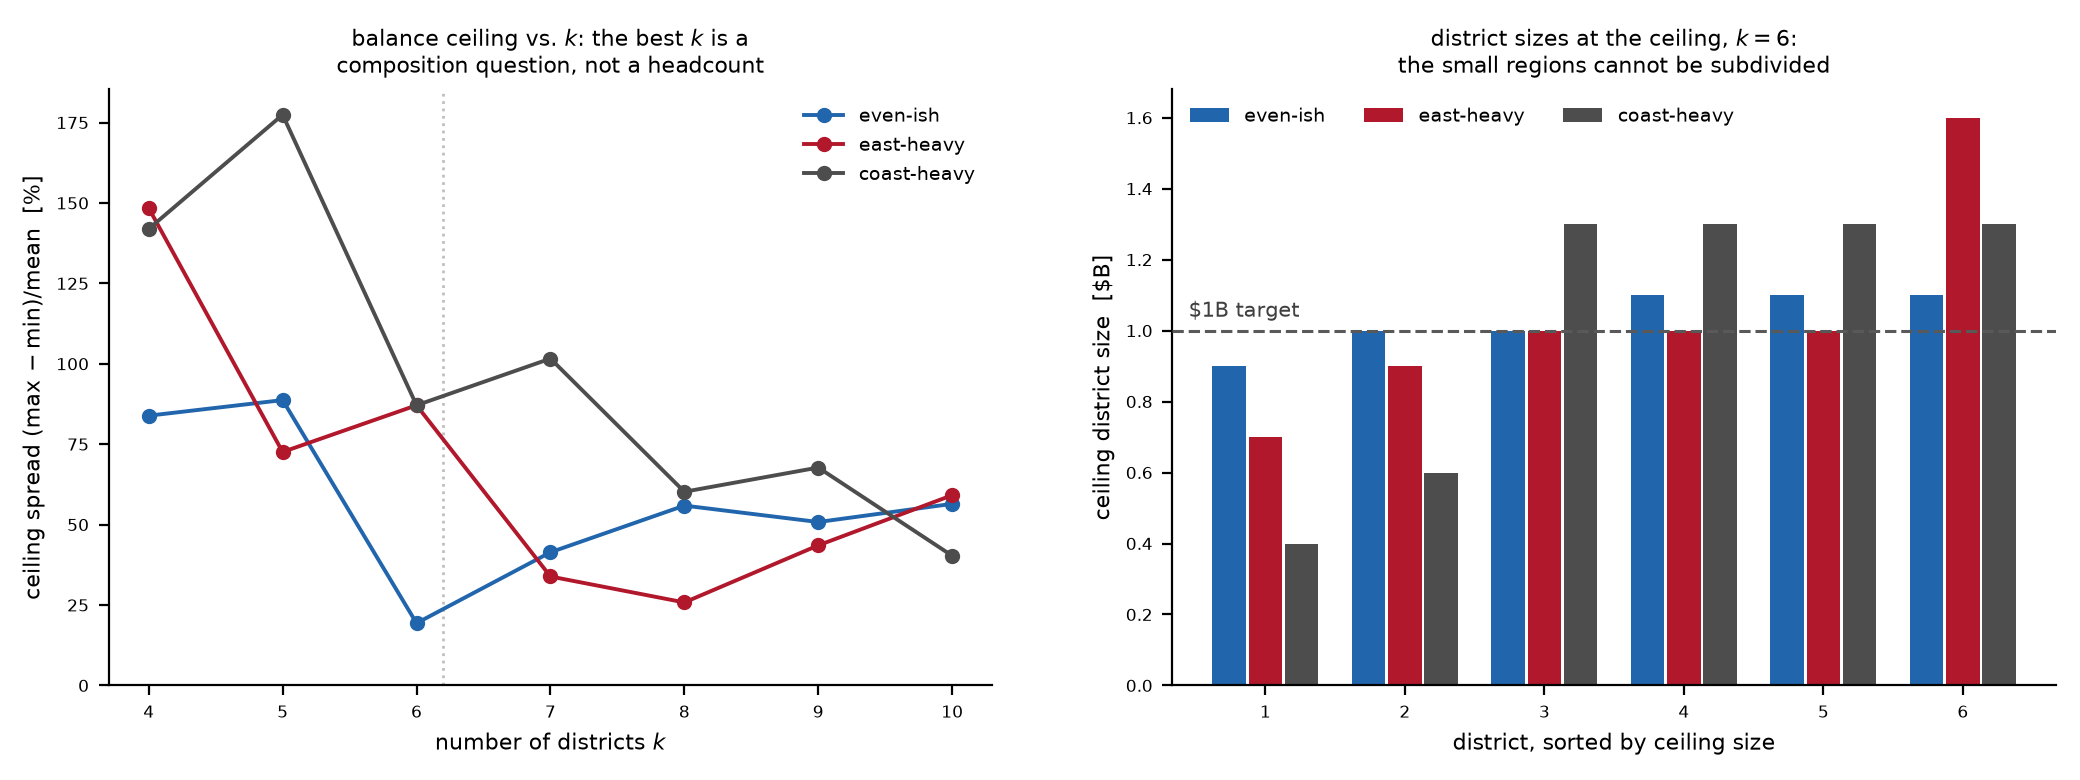
\includegraphics[width=\textwidth]{ceiling.png}
\caption{The balance ceiling of Proposition~\ref{prop:ceiling} on three illustrative
splits of the $\$\chTotalB$B footprint across its $\chComponents$ components.
\emph{Left:} ceiling spread against $k$; the dotted line marks the $k$ implied by a
$\$\chTargetB$B target. The curves cross repeatedly --- there is no composition-free
best $k$. \emph{Right:} the $\chKAtTarget$ ceiling district sizes under each split,
sorted, against the $\$\chTargetB$B target. Under \chCoastLabel{} two districts are pinned
below $\$0.6$B by components too small to divide, while the coastal districts sit at
$\$\chCoastkSixMax$B; no contiguous draw can improve on this picture, only fall short of
it.}
\label{fig:ceiling}
\end{figure}

\section{Stage-1 formulation}\label{sec:formulation}

Stage~1 is a balanced contiguous districting problem, the classical shape in the sales-
and political-districting literatures \citep{hess1971,zoltners2005,riosmercado2009,duque2011}.
Written in the $n$-way form the harness already carries, with $y_{z,i}=1$ iff zip $z$ is
assigned to candidate $i$:
\begin{equation}\label{eq:milp}
\begin{aligned}
\max\;\; & \sum_i \zeta_i \;-\; \rho \sum_{e\in E} w_e\\
\text{s.t.}\;\;
& \sum_{i\in\mathrm{cand}(z)} y_{z,i} = 1 && \forall z\in Z,\\
& g_i \;\le\; \sum_z u_i(z)\, y_{z,i} && \forall i,\\
& \zeta_i \;\le\; \log \hat g_i + \frac{\bigl(\sum_z u_i(z) y_{z,i}\bigr)-\hat g_i}{\hat g_i}
   && \forall i,\ \forall \text{ tangent points } \hat g_i>0,\\
& \sum_{w\in C} y_{w,i} \;\ge\; y_{u,i} + y_{v,i} - 1
   && \forall i,\ \forall u,v,\ C \text{ a } u,v\text{-separator},\\
& y_{z,i}\in\{0,1\}.
\end{aligned}
\end{equation}

Four notes, each of which is a trap already paid for in the two-player programme.

\begin{itemize}
\item \textbf{$\le$, not $=$, on the gains.} The objective is increasing in $g_i$ through
the logs, so $g_i\le\sum_z u_i(z)y_{z,i}$ is tight at every optimum. Writing it as an
equality lets presolve multi-aggregate the gain variables out of the transformed problem,
after which no in-callback incumbent can be posted at all. Relatedly, dual presolve
reductions must be disabled: they count variable locks over the constraints presolve can
\emph{see}, and lazily separated rows are not there yet.
\item \textbf{The tangents are outer approximation, one family per representative.} Each
supports $\zeta_i\le\log g_i$ at $\hat g_i$ and is valid everywhere, so the tangent set is a
relaxation and the master's value is a genuine upper bound \citep{duran1986,fletcher1994};
a certificate is the moment the incumbent meets it. The $\varepsilon$-certified
piecewise-linear alternative \citep{vielma2011,caragiannis2019} trades the loop for a
bounded a-priori error. The gain lower bound must come from the incumbent, never from an
absolute floor like $10^{-9}$: the log's gradient there is $10^{9}$ and destabilises the LP.
\item \textbf{The separator cuts are root-free and uniform.} If a feasible allocation puts
both $u$ and $v$ with representative $i$, it contains an $i$-path between them; every such
path meets the separator $C$, so some $w\in C$ has $y_{w,i}=1$. If either endpoint is
elsewhere the right-hand side is $\le0$ and the cut is slack. Validity does not depend on
how $u$, $v$, $C$ were chosen, which is what lets the same construction separate fractional
points. Crucially, \emph{no root is fixed}: a rooted formulation is unsound on a
disconnected graph, since it forces growth toward a vertex other components cannot reach,
and its ``dual bound'' can sit strictly below feasible allocations already visited --- not
a corner case on a footprint that is disconnected by design. Encoding alternatives ---
single-commodity flow from a root \citep{shirabe2005}, lazily separated cuts
\citep{validi2021,validibuchanan2022}, cutting-plane aggregation \citep{oehrlein2017} ---
differ mainly in how they pay for this.
\item \textbf{Both cut families belong in \emph{one} branch-and-cut tree.} Outer
approximation converges by the Duran--Grossmann argument and lazy feasibility cuts by
combinatorial Benders \citep{hooker2003,codato2006}; in a multi-tree loop that restarts a
fresh MILP after each round, the two iteration counts \emph{multiply}. A single tree with
both families separated lazily at nodes \citep{quesada1992,bonami2008,validi2021} keeps one
globally valid dual bound throughout.
\end{itemize}

\paragraph{The symmetry hazard, and the Hess remedy.}
Formulation \eqref{eq:milp} inherited its index $i$ from the merger problem, where
representatives are named and distinguishable. In stage~1 they are not: the $k$ districts
are \emph{anonymous}, so any permutation of the labels maps a feasible solution to an
equally good one and branch-and-bound must re-derive and re-prune $k!$ copies of every
subtree --- $720$ copies at $k=\chKAtTarget$. The standard remedy is the centre-based
formulation of \citet{hess1971}: introduce $k$ \emph{centres} chosen from the units, index
districts by their centre, and require $y_{z,c}\le y_{c,c}$. Labels are then pinned by
geography and the symmetry is broken by construction, which is why the districting
literature uses it \citep{zoltners2005,salazaraguilar2011,rosmercado2012}. The centre choice
is itself a decision and interacts with contiguity, so this buys pruning with a larger
model, not for free.

\paragraph{If $\chZips$ units proves too large.}
In increasing order of concession: per-component solves at ${\sim}500$ zips, which the
disconnection already licenses; pre-aggregation to clusters or county/CBSA level, then
disaggregation \citep{karypis1998}; $\varepsilon$-certified acceptance at the harness's
existing tier-2 tolerance; and last a heuristic with a reported bound, for which
Proposition~\ref{prop:ceiling} supplies the dual side for free and column generation or
recombination sampling the primal \citep{gurnee2021,deford2021,bozkaya2003}. Connected fair
division is NP-hard already for two agents with identical valuations
\citep{deligkas2021}, so exactness with certificates --- not a closed form --- is the
realistic target; see \citet{bouveret2017,bilo2022,suksompong2019} for the
fair-division-on-graphs setting and \citet{bei2022} for the only price-of-connectivity
bounds available (none is known for Nash welfare).

\section{Open questions}\label{sec:open}

These are modelling decisions, not implementation gaps. Each changes the answer.

\begin{enumerate}
\item \textbf{Empty bundles.} Insisting that every representative receive a non-empty
contiguous bundle is a real and possibly infeasible constraint, and a single $g_i=0$ sends
$\sum_i\log g_i$ to $-\infty$. The standard treatment is lexicographic --- maximise the
count of representatives with positive utility, then maximise Nash welfare among them
\citep{caragiannis2019} --- and is the recommendation.
\item \textbf{Directionality of $\theta$.} If capture depends on \emph{which}
representative is displaced, the single scalar becomes $\theta_{i\leftarrow j}$ and the
identification problem grows from one parameter to $O(n^2)$ --- and $\theta$ is already the
one parameter resting on unfinished causal work.
\item \textbf{The brute-force acceptance tier.} The harness accepts a method partly on
matching exhaustive enumeration at $n\le20$; at three candidates per zip that is
$3^{20}\approx3.5\times10^9$ leaves. The tier must be re-cut by candidate-weighted size
$\prod_z|\mathrm{cand}(z)|\le10^6$--$10^7$. This weakens a stated acceptance criterion and
needs sign-off, not a quiet redefinition.
\item \textbf{Who owns an untapped or vacant zip?} Under $\mathrm{cand}(z)=\{i:S_i(z)>0\}$
neither class has a candidate, yet both carry opportunity and both hold the graph together
(the ``zero-value glue'' of failure regime~(d)), so dropping them changes connectivity.
Options: leave unallocated, assign by adjacency, or widen candidacy for these zips only.
\emph{For the national channel the question largely dissolves}: stage~1 partitions the whole
footprint on opportunity alone, so every zip lands somewhere by construction, and candidacy
re-enters only at stage~2 through \eqref{eq:gij}.
\item \textbf{The filler capture mode.} $\cfree\in\{c_2,c_1,\lambda\}$ per
Section~\ref{sec:free}; \texttt{full} ($c_1$) is the recommendation. The three modes give
materially different maps, so this is a decision and not a default.
\end{enumerate}

\bibliographystyle{plainnat}
\bibliography{references}

\end{document}
